

\section{Ablation}
\begin{figure}[h]
    \centering
    \begin{subfigure}[b]{0.48\textwidth}
        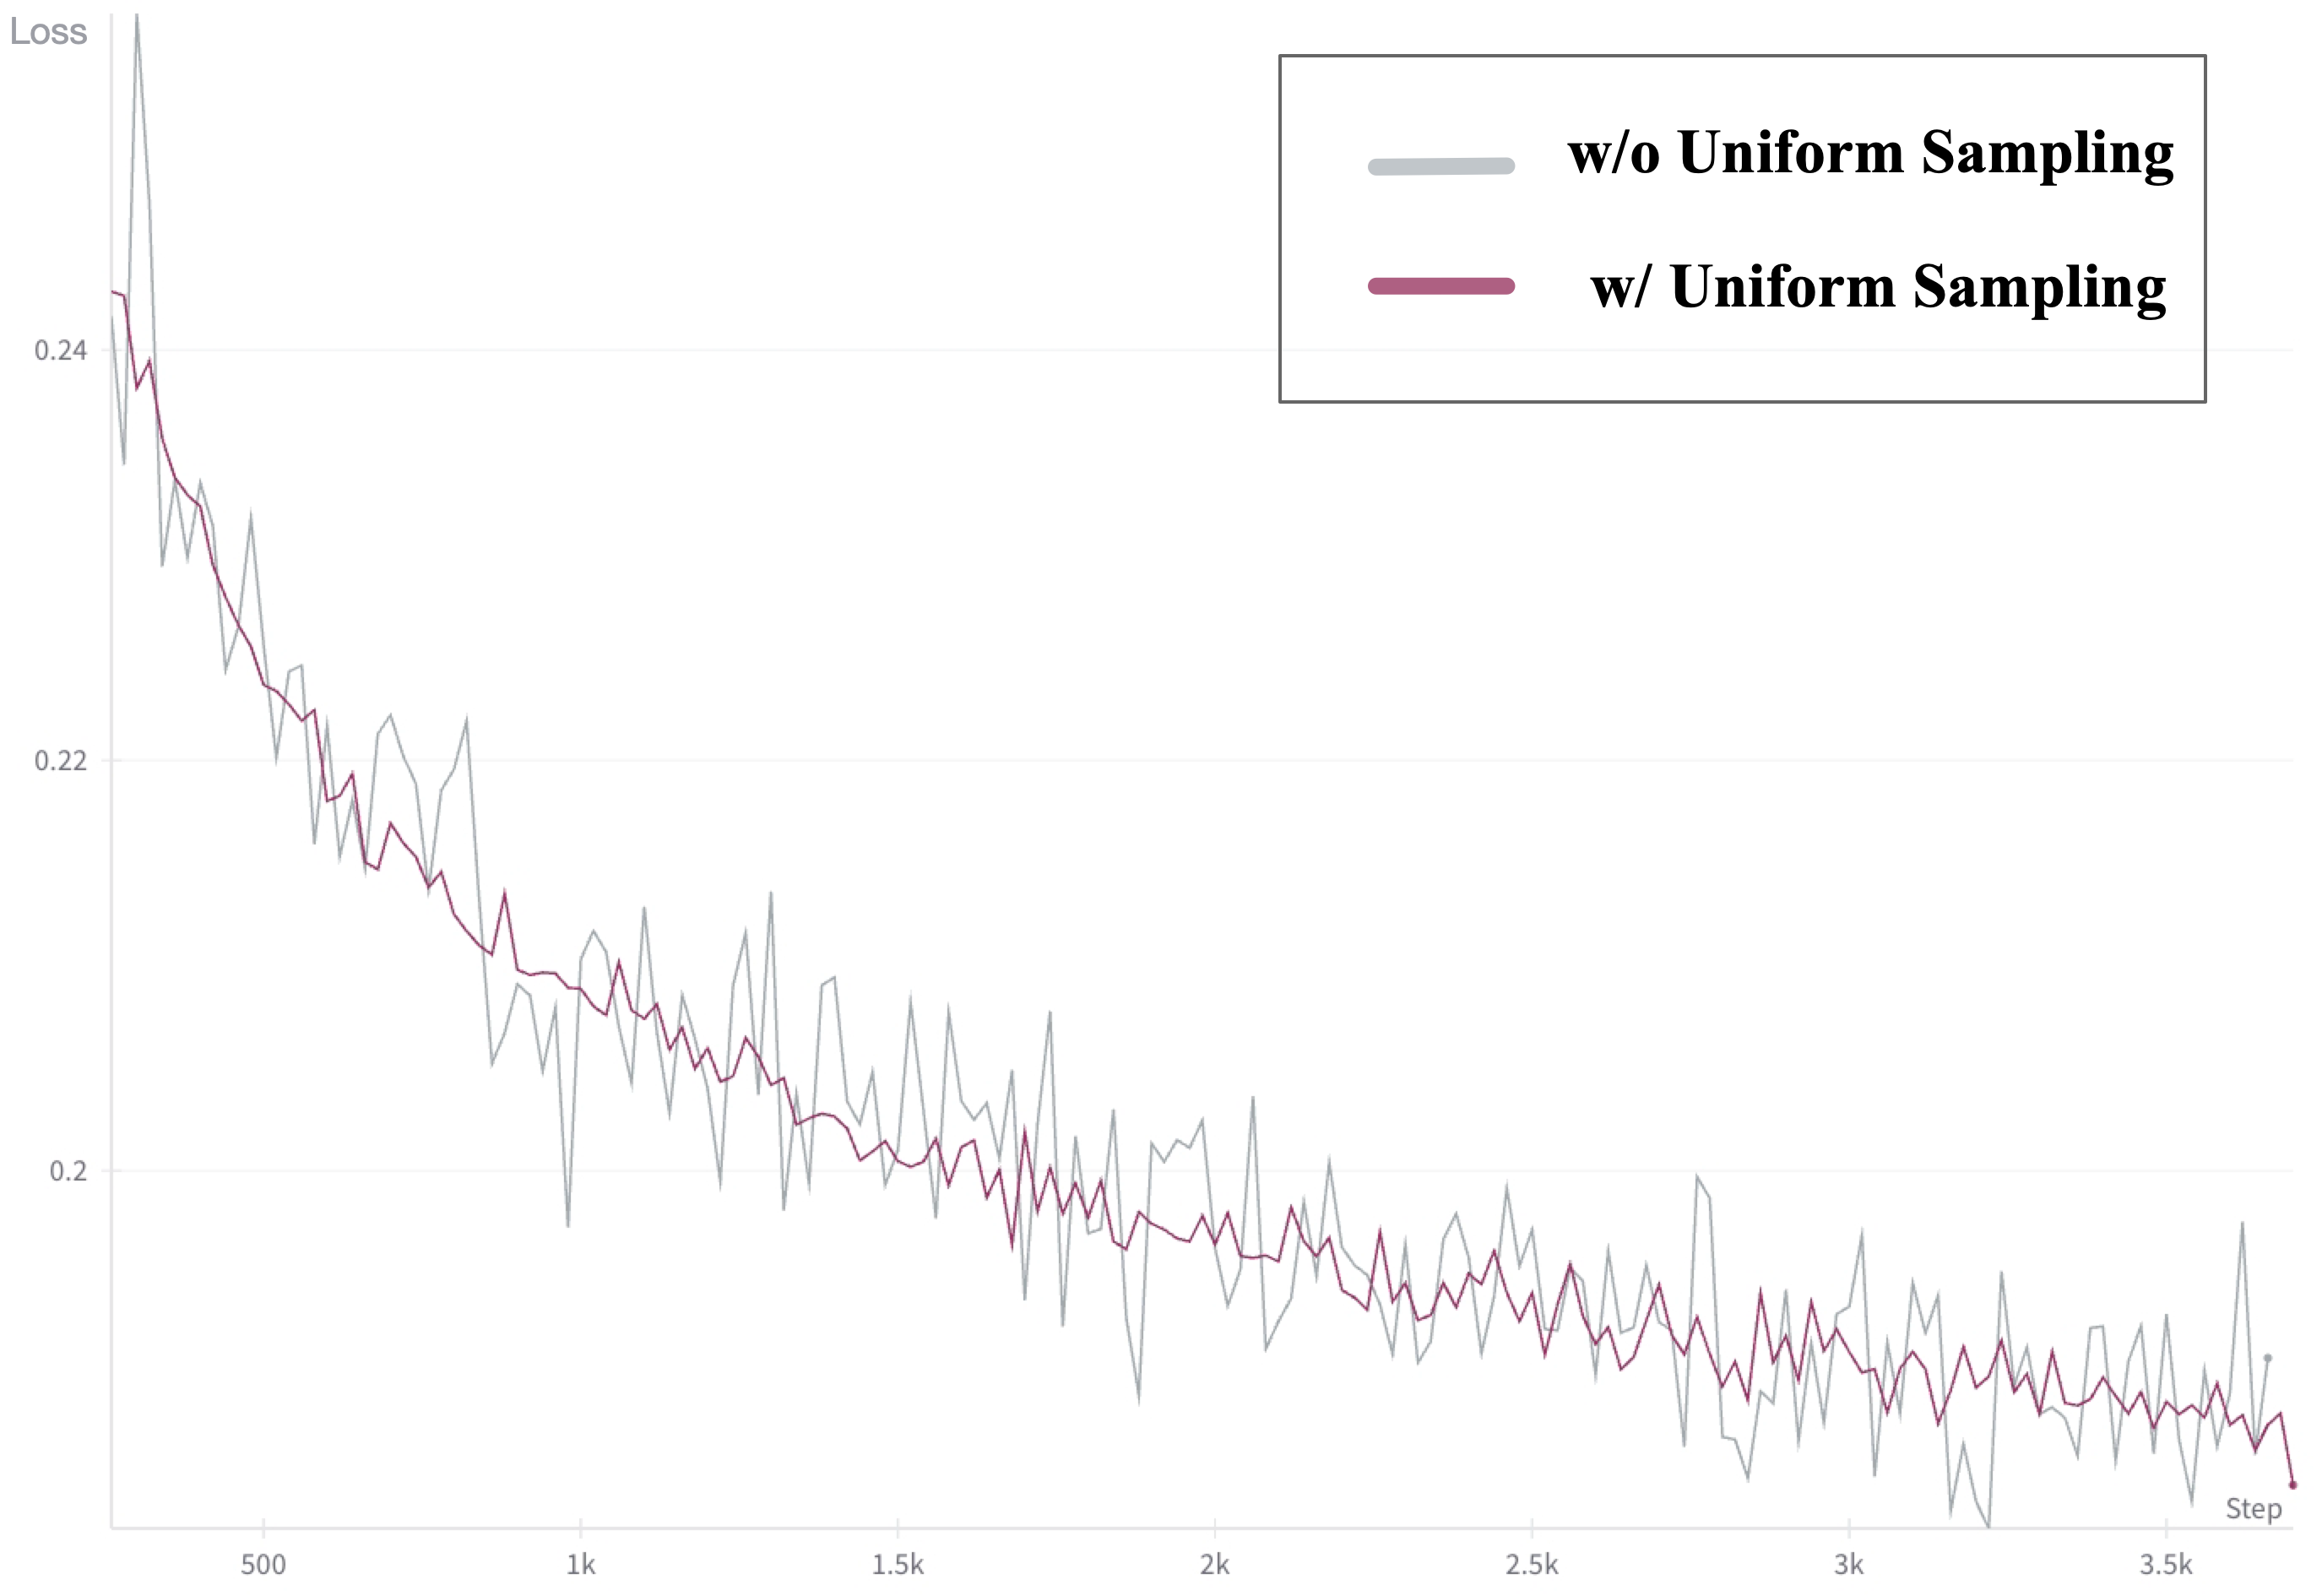
\includegraphics[width=\textwidth]{images/ab_us.png}
        \caption{Bottom aligned}
        \label{fig:a}
    \end{subfigure}
    \begin{subfigure}[b]{0.48\textwidth}
        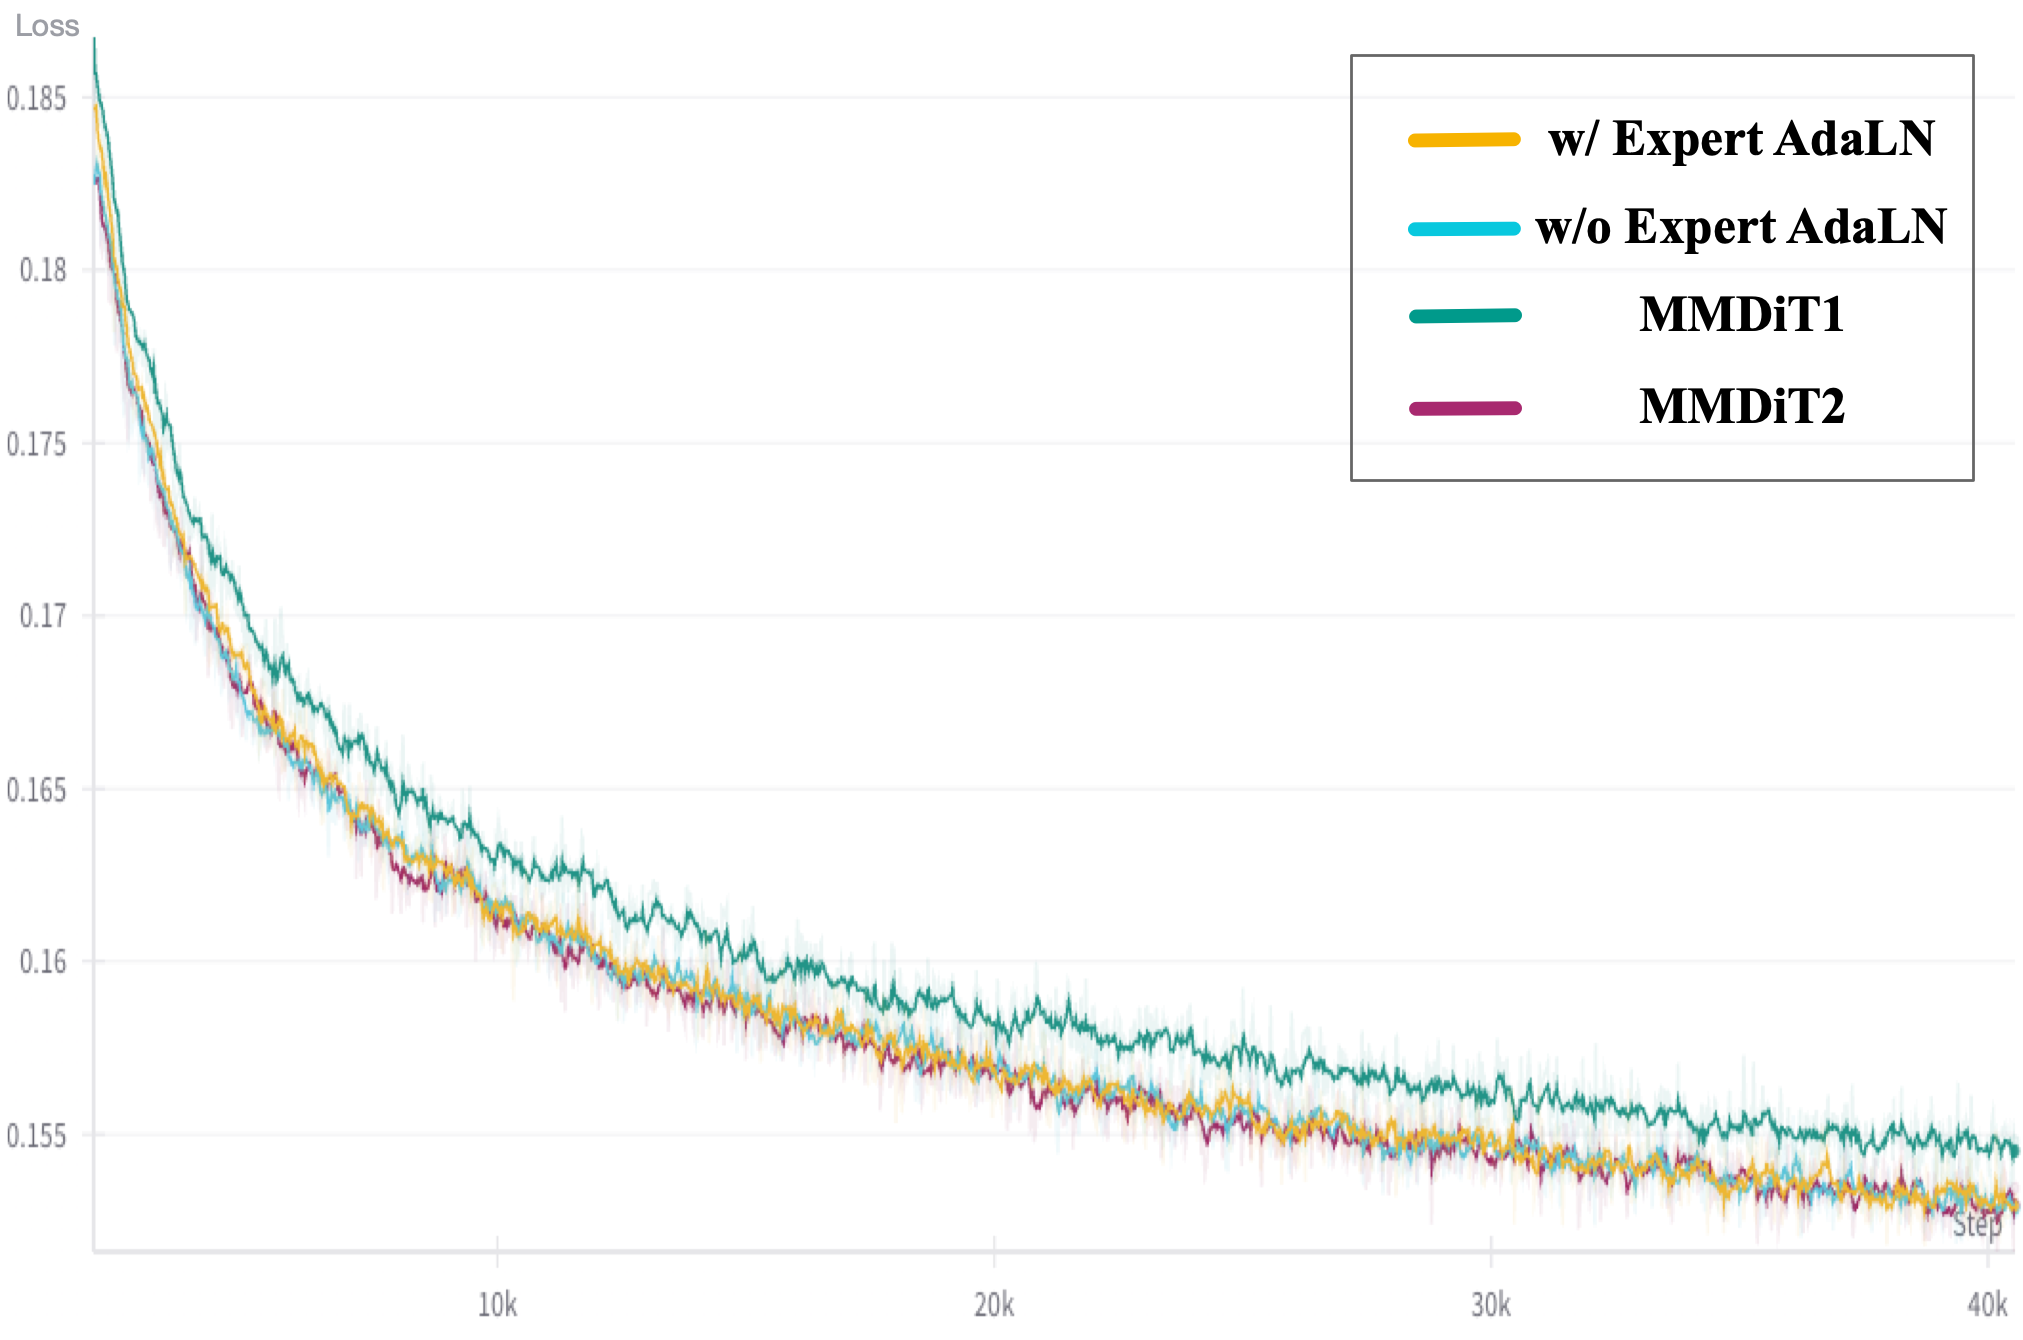
\includegraphics[width=\textwidth]{images/ab_ex.png}
        \caption{Bottom aligned}
        \label{fig:b}
    \end{subfigure}
    \begin{subfigure}[b]{0.50\textwidth}
        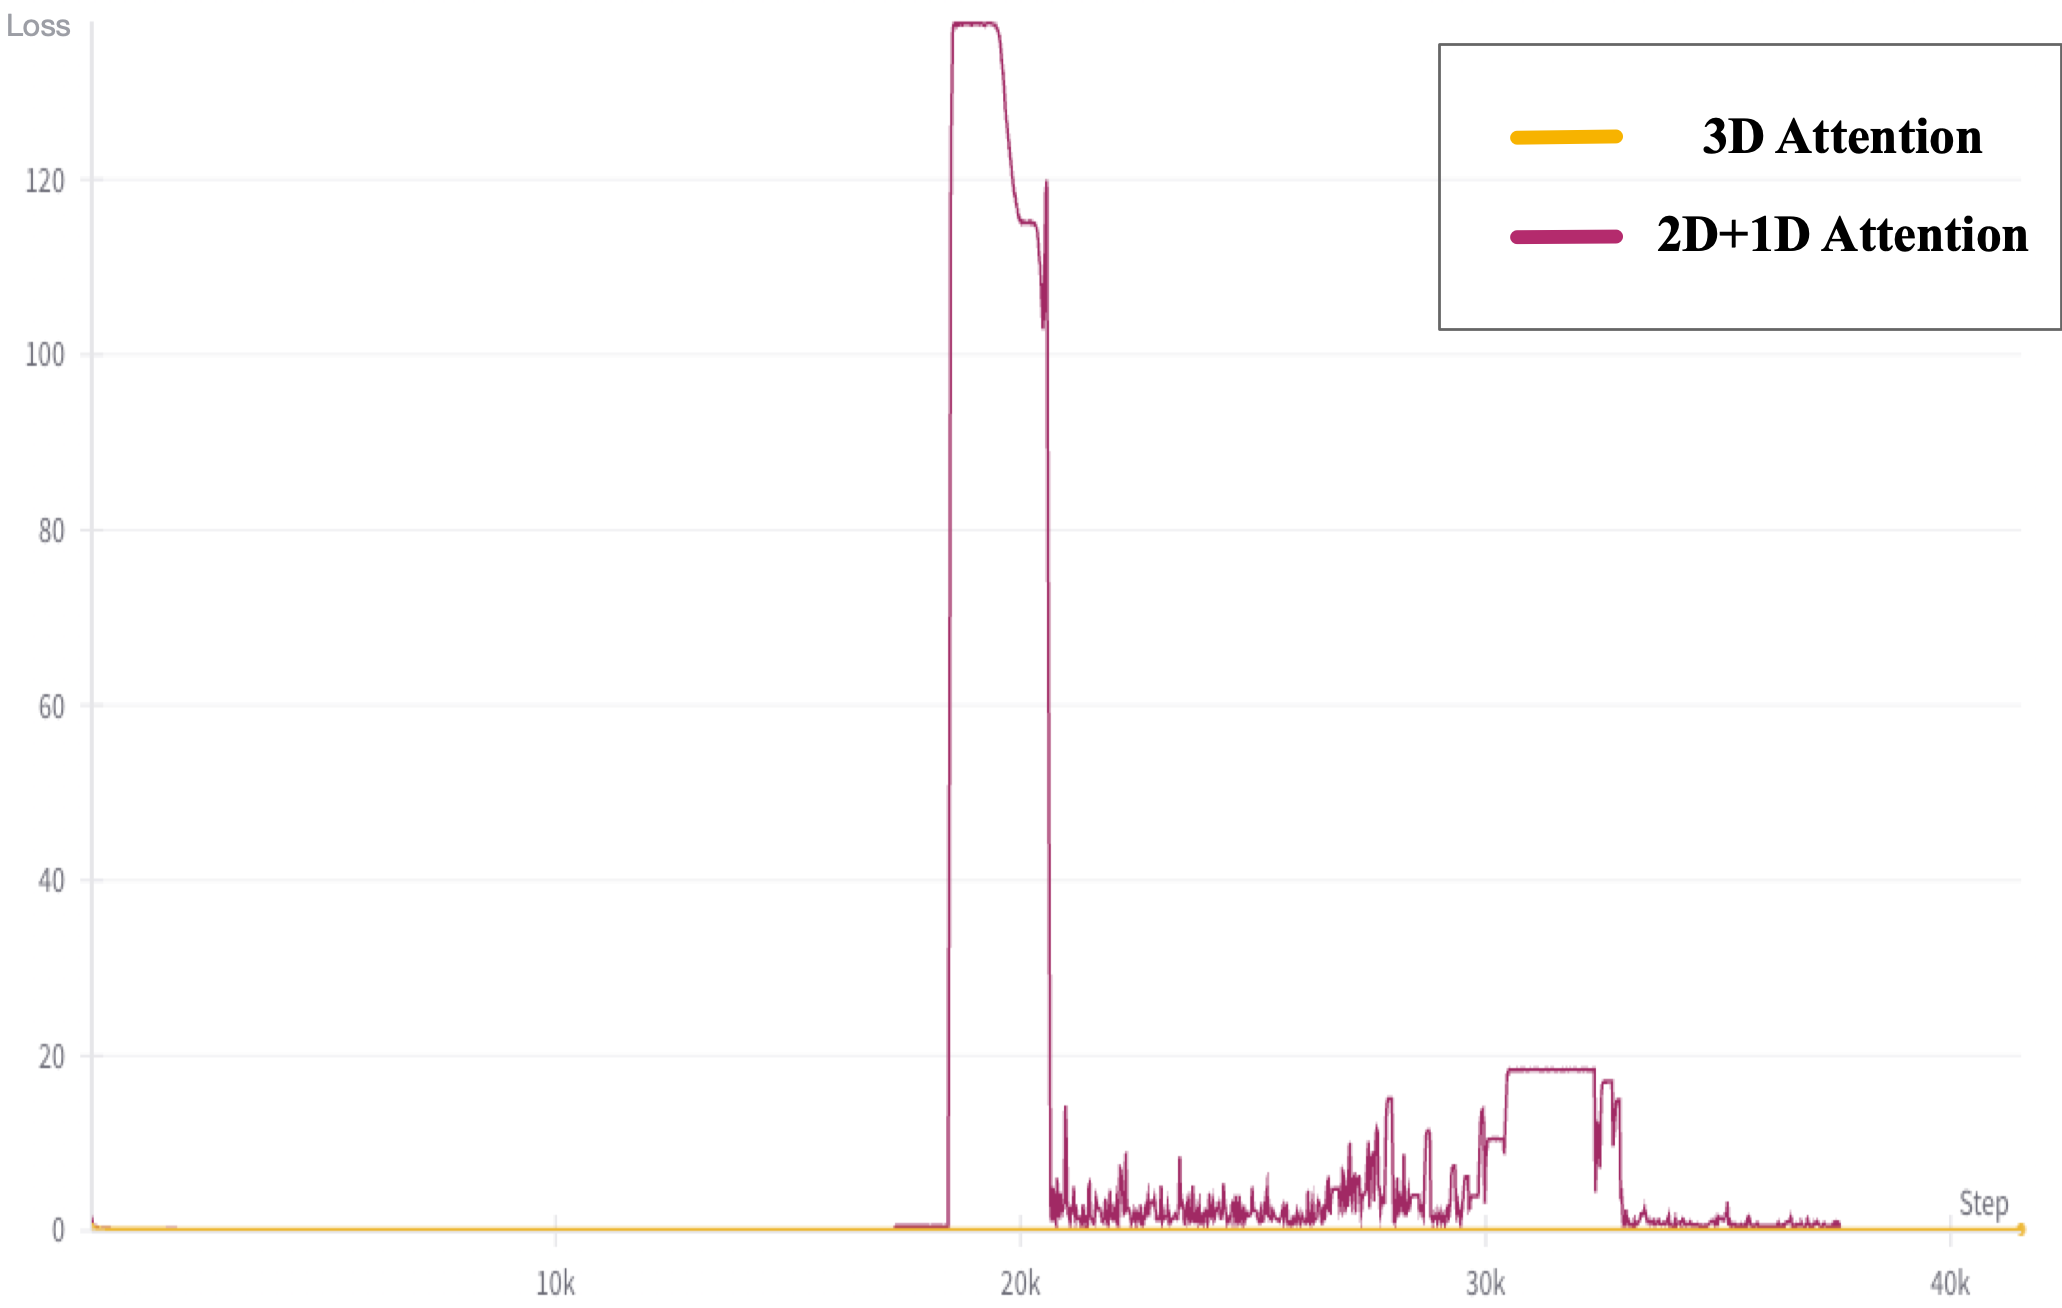
\includegraphics[width=\textwidth]{images/ab_rl.png}
        \caption{Bottom aligned}
        \label{fig:c}
    \end{subfigure}
    \begin{subfigure}[b]{0.46\textwidth}
        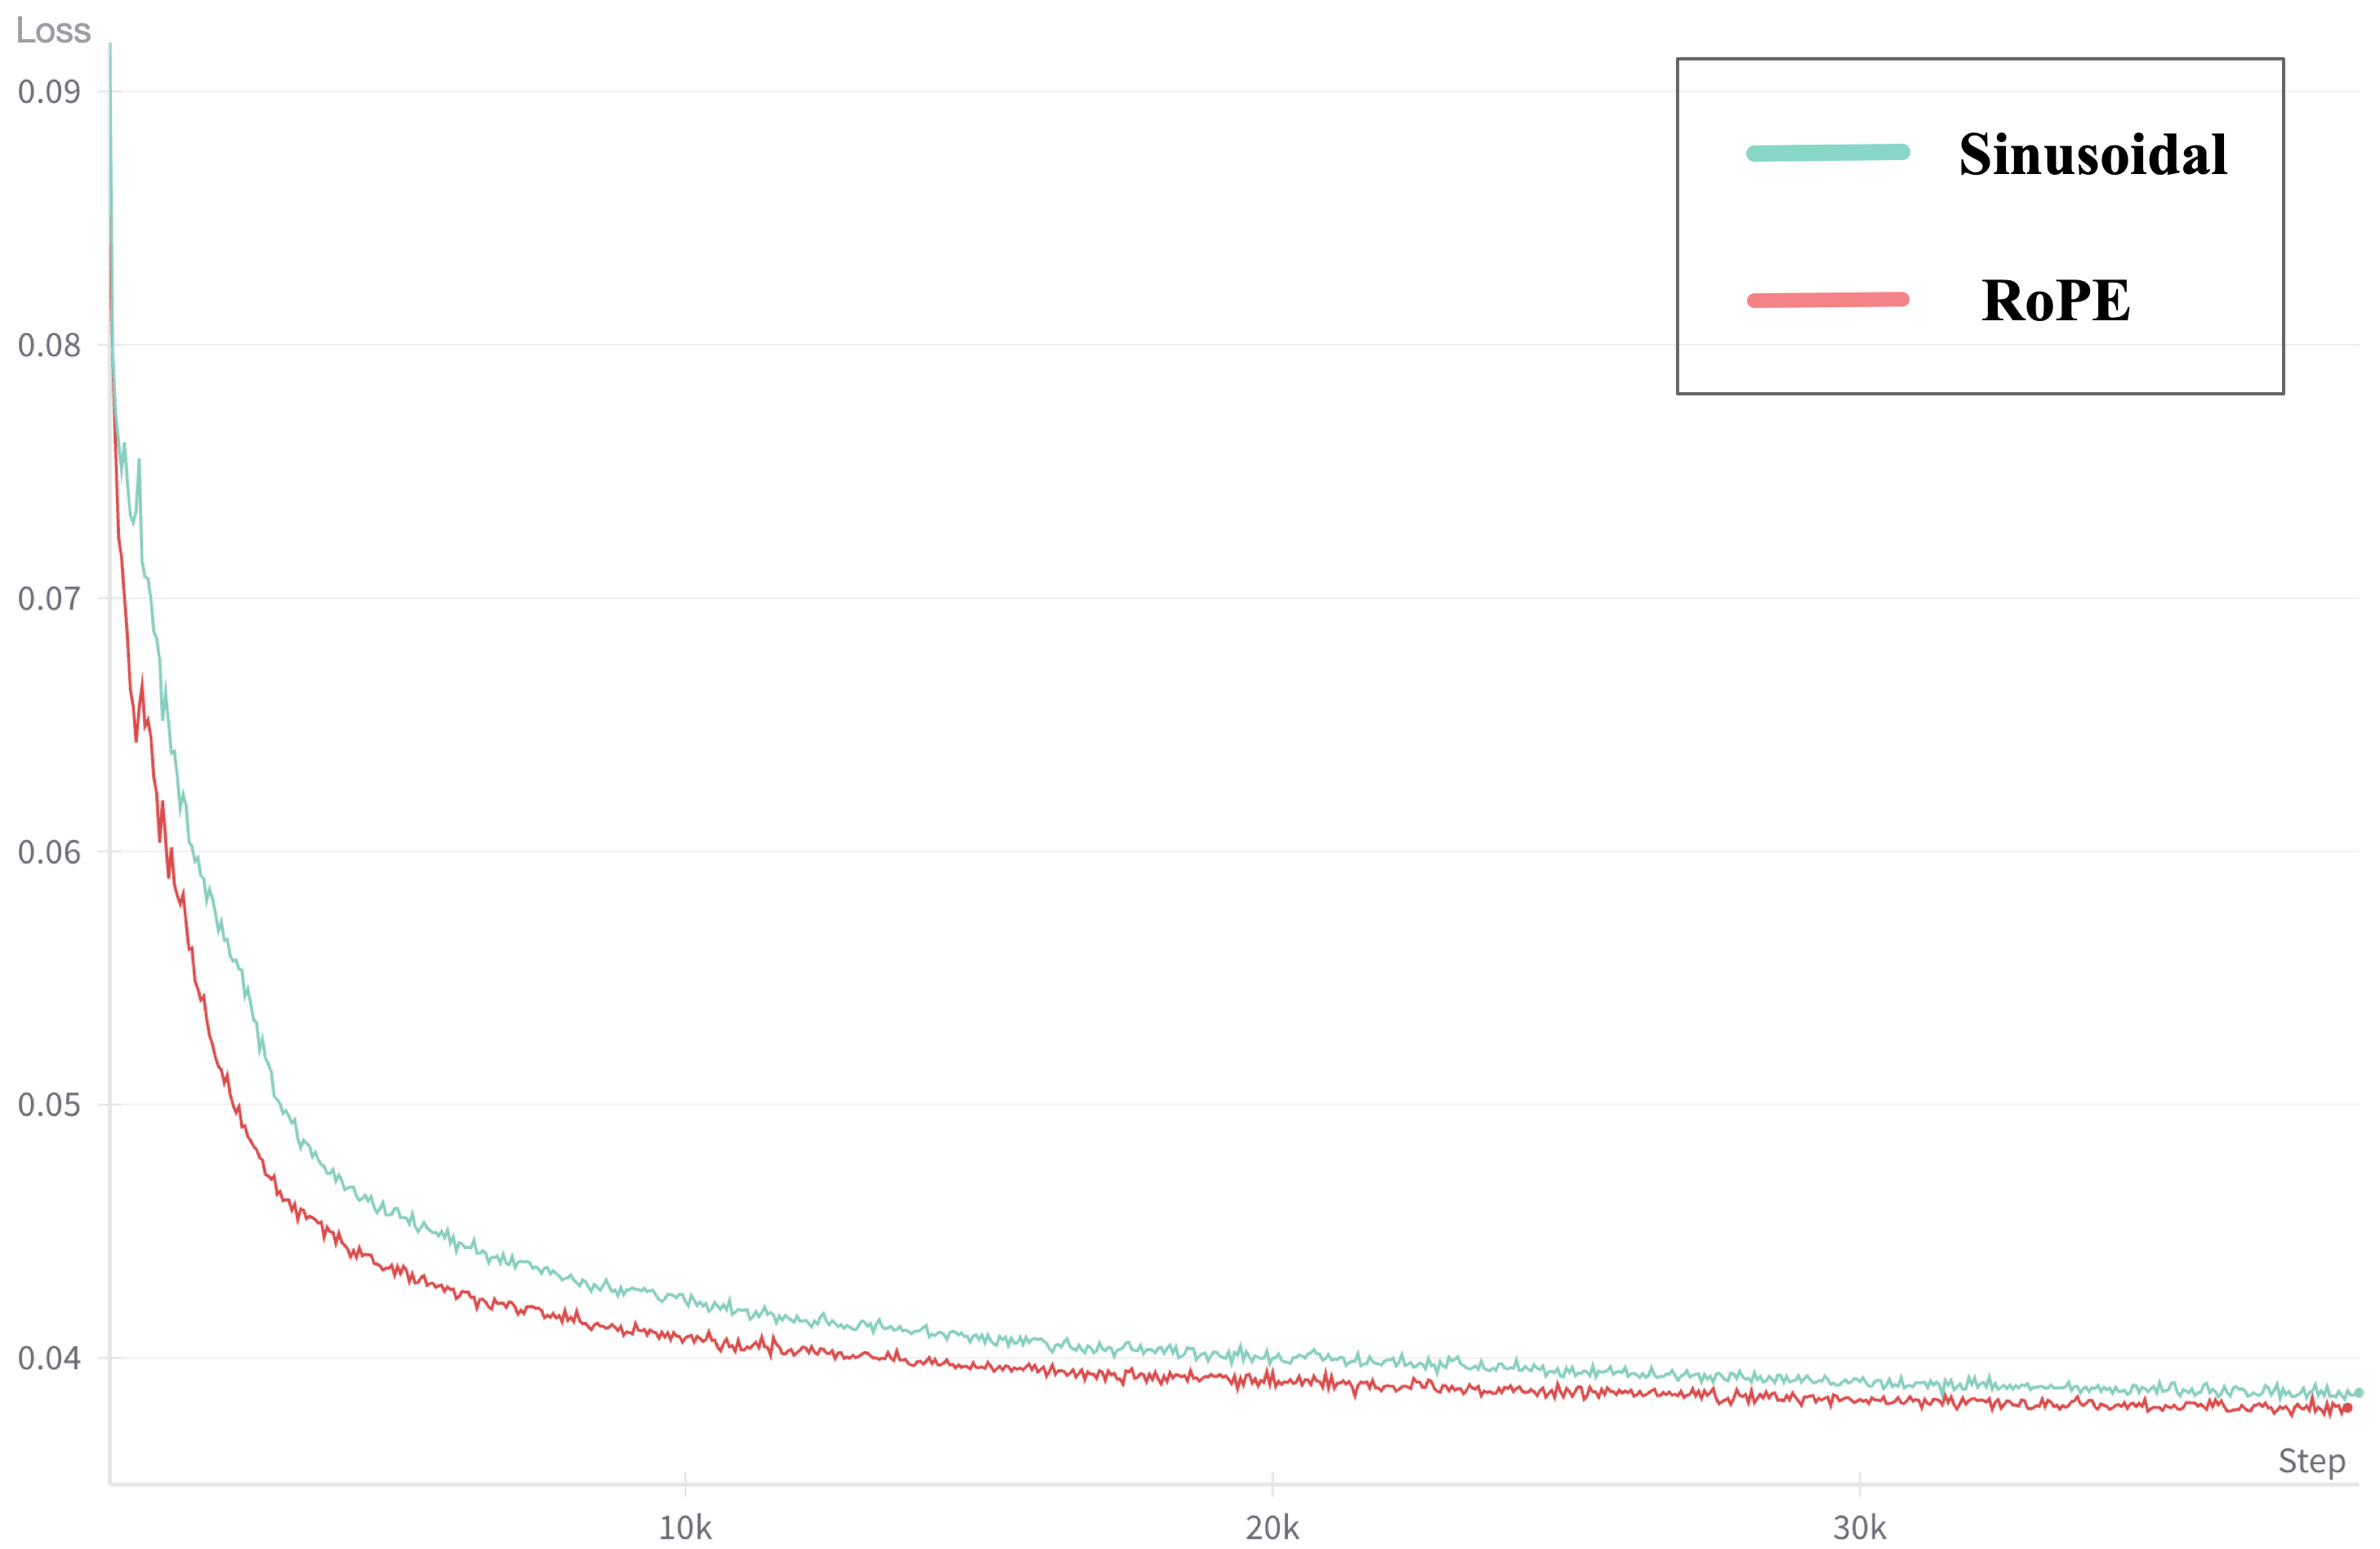
\includegraphics[width=\textwidth]{images/ab_sr.png}
        \caption{Bottom aligned}
        \label{fig:d}
    \end{subfigure}
    \caption{Overall caption for the figure.}
    \label{fig:subfigures}
\end{figure}

We conducted ablation studies on some of the designs mentioned in Section~\ref{sec:model} to verify their effectiveness.


\subsection{Position Embedding}
First, we compared 3D RoPE with sinusoidal absolute position encoding. As shown in Figure~\ref{fig:d}, the loss curve using 3D RoPE converges significantly faster than that with sinusoidal encoding.
Then we compared the use of 3D RoPE alone with the combination of 3D RoPE and learnable absolute position embedding. As shown in Figure~\ref{fig:c}, the loss curves of both methods converge almost identically. For simplicity, we chose to use 3D RoPE alone.

\subsection{Expert Adaptive Layernorm}
We experimented with different ways of incorporating experts: expert LayerNorm and MLP, and expert Layernorm only. Our experiments found that adding expert MLP does not effectively accelerate the model's convergence (Figure~\ref{fig:b}). To reduce the model parameters, we only chose to use expert adaptive Layernorm.